\section{SpaceX}

{
\logo{}
\subsection{Why SpaceX exists}

\begin{frame}
\frametitle{Why SpaceX Exists}

    \begin{columns}
        \begin{column}{45mm}
        The ultimate goal : \\Colonise Mars (no less)
        \end{column}
        \begin{column}{65mm}
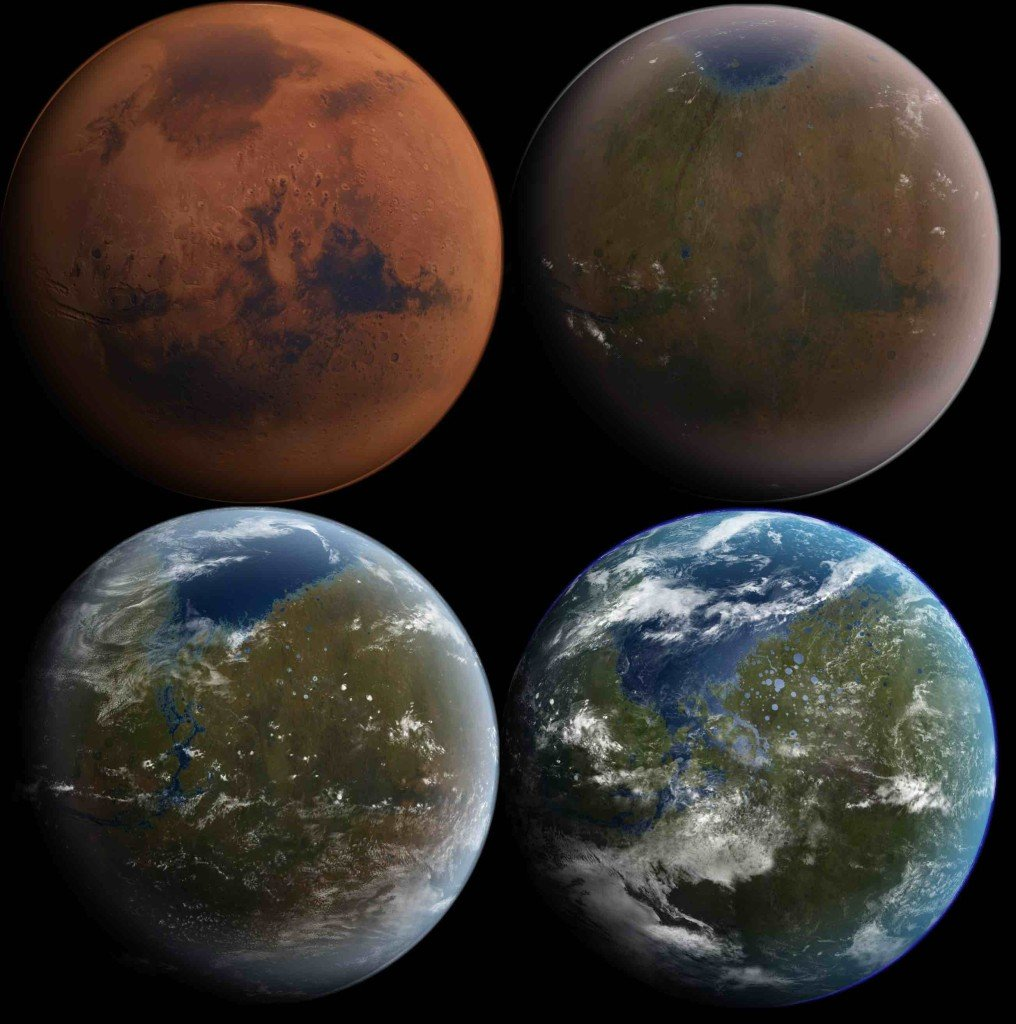
\includegraphics[width=65mm]{images/mars_transition}
        \end{column}
    \end{columns}
\end{frame}
}


\subsection{The Problem}

\begin{frame}
    \frametitle{The Problem}
    \begin{itemize}
        \item 1M people needed for autonomous colony \pause
        \item current Mars shuttle holds 6 \pause
        \item costs 50 M\$ per passenger
    \end{itemize}
\end{frame}

\begin{frame}
    \frametitle{The Solution}
    \begin{enumerate}
        \item Learn rocket science
        \pause
        \item Make cost-effective rockets
        \pause
        \item Put payloads in orbit $\rightarrow$ experience and profit
        \pause
        \item Bring Mars flight ticket to 500 000 \$
        \pause
        \item Send people by batches of 100
    \end{enumerate}
\end{frame}

\subsection{SpaceX History}

\begin{frame}
    \frametitle{SpaceX History}

    \begin{itemize}
        \item 2006 - first launch  $\rightarrow$ failure
        \item 2007 - second launch $\rightarrow$ failure
        \item 2008 - third launch  $\rightarrow$ failure

    \end{itemize}
    \vspace{1em}
    \pause

    september 2008\\
    last try before running out of funds\\
    \begin{itemize}
        \item success $\rightarrow$ 1.6 B\$ contract with NASA
    \end{itemize}
\end{frame}

\subsection{SpaceX's Technology}

{
    \logo{}

\begin{frame}
    \frametitle{SpaceX's Current Technology}
    \begin{columns}
        \begin{column}{60mm}
            The merlin engine :\\
            \vspace{1em}
            \begin{itemize}
                \item mass : 440 kg
                \item thrust : 716 kN ($\simeq$73 Tons)
                \item thrust-to-weight ratio : 165.9
            \end{itemize}
        \end{column}
        \begin{column}{45mm}
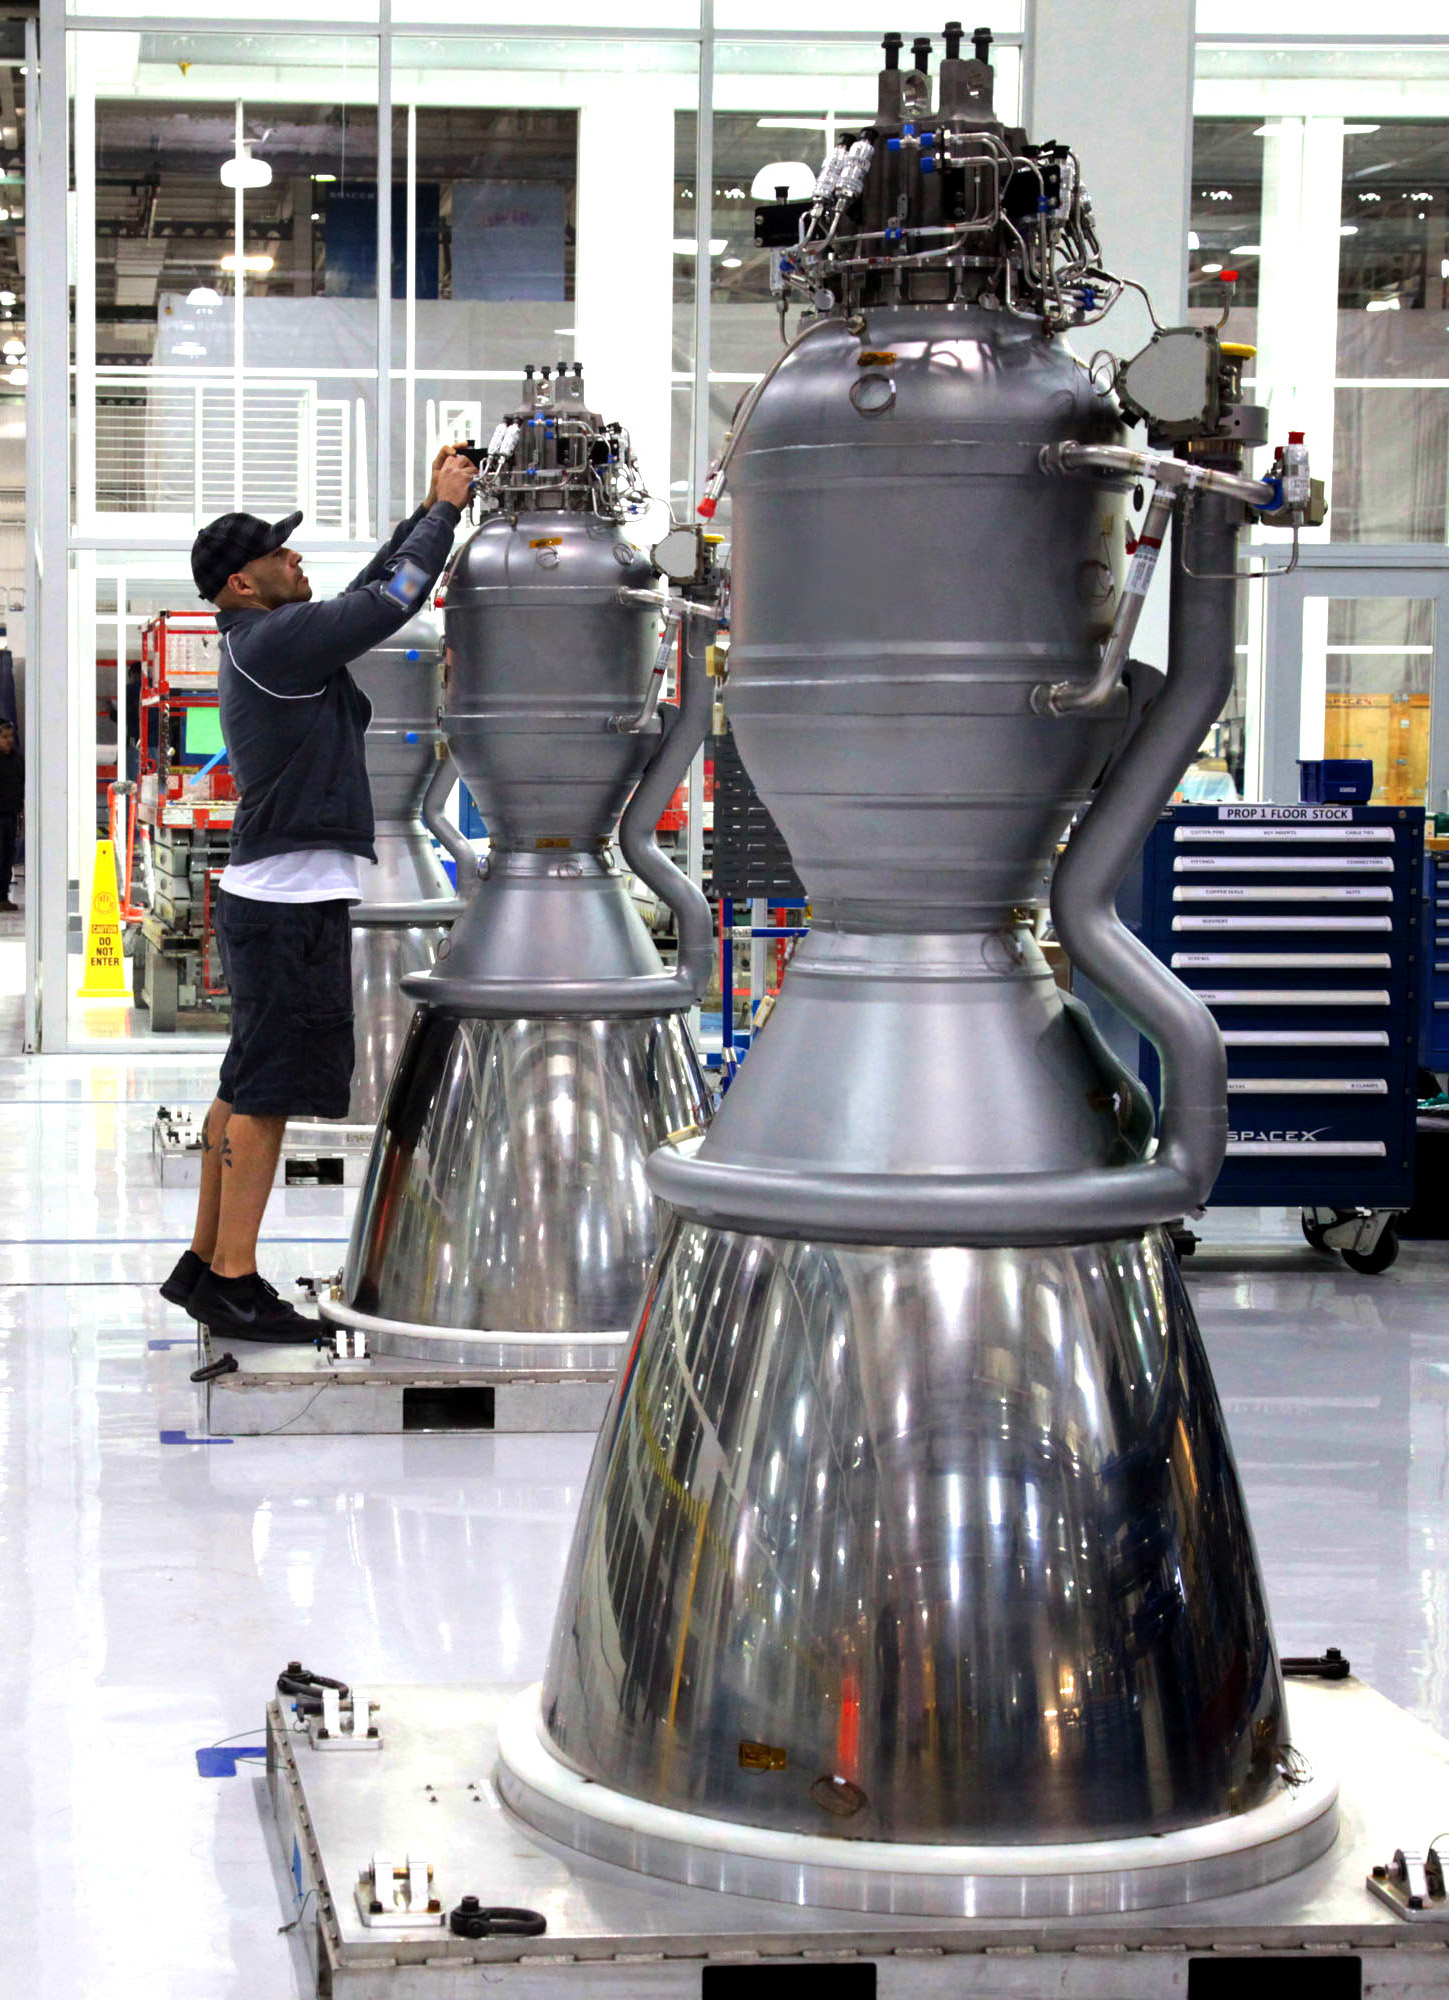
\includegraphics[width=48mm]{images/shiny_merlin}
        \end{column}
    \end{columns}
\end{frame}

\begin{frame}
    \frametitle{SpaceX's Current technology}
    \begin{columns}
        \begin{column}{60mm}
            The falcon 9 :\\
            \vspace{1em}
            \begin{itemize}
                \item 68m high
                \item 13 tons of payload to LEO
                \item active since 2010
                \item uses 9 Merlins \\(hence the name)
            \end{itemize}
        \end{column}
        \begin{column}{50mm}
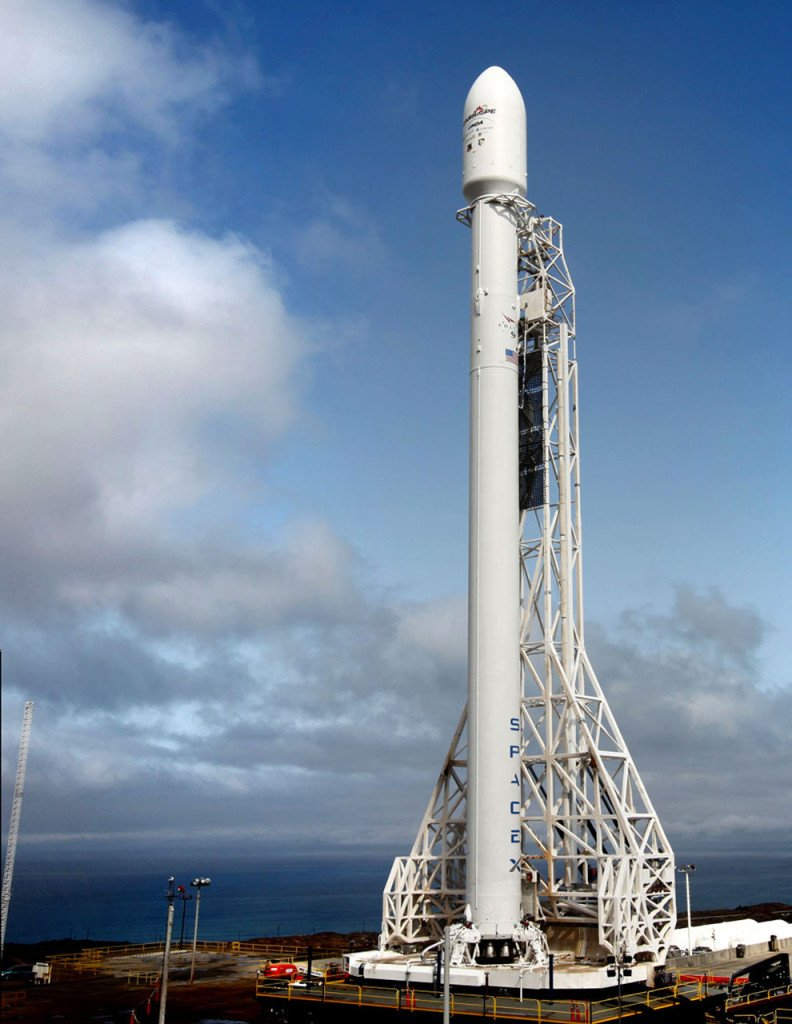
\includegraphics[height=66mm]{images/falcon9}
        \end{column}
    \end{columns}
\end{frame}

\begin{frame}
    \frametitle{SpaceX's Current technology}
    \begin{columns}
        \begin{column}{50mm}
            Dragon :\\
            \vspace{1em}
            \begin{itemize}
                \item car-sized
                \item used for resupply mission to ISS
                \item contract with NASA for 12 Dragons
            \end{itemize}
        \end{column}
        \begin{column}{65mm}
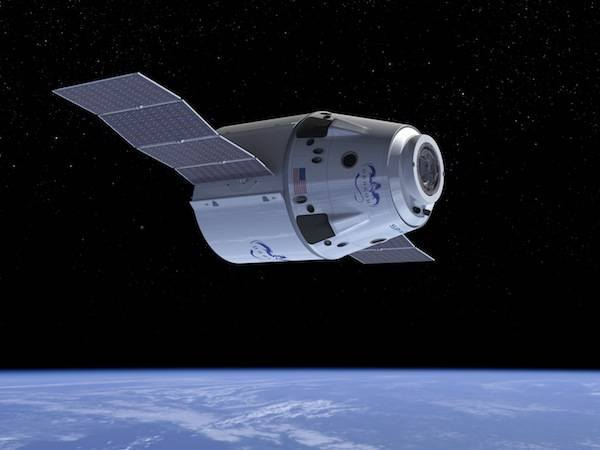
\includegraphics[height=50mm]{images/dragon}
        \end{column}
    \end{columns}
\end{frame}
}

\begin{frame}
    \frametitle{SpaceX's Future Technology}
    \begin{itemize}
        \item Send 100 people to Mars at a time
        \item Improve cost-effectiveness
        \item Make rockets reusable
    \end{itemize}

\end{frame}

\begin{frame}
    \frametitle{In practice}
    \begin{columns}
        \begin{column}{55mm}
            Achieve cost-efficiency by :
            \begin{itemize}
                \item<1-> In-house manufacturing 
                \item<2-> Innovative ideas (reusability)
                \item<3-> Using current technology
                \item<4> Saving on catering
                \item<6-> Price reaches 500 000 \$ 
            \end{itemize}
        \end{column}
        \begin{column}{65mm}
            \only<7->{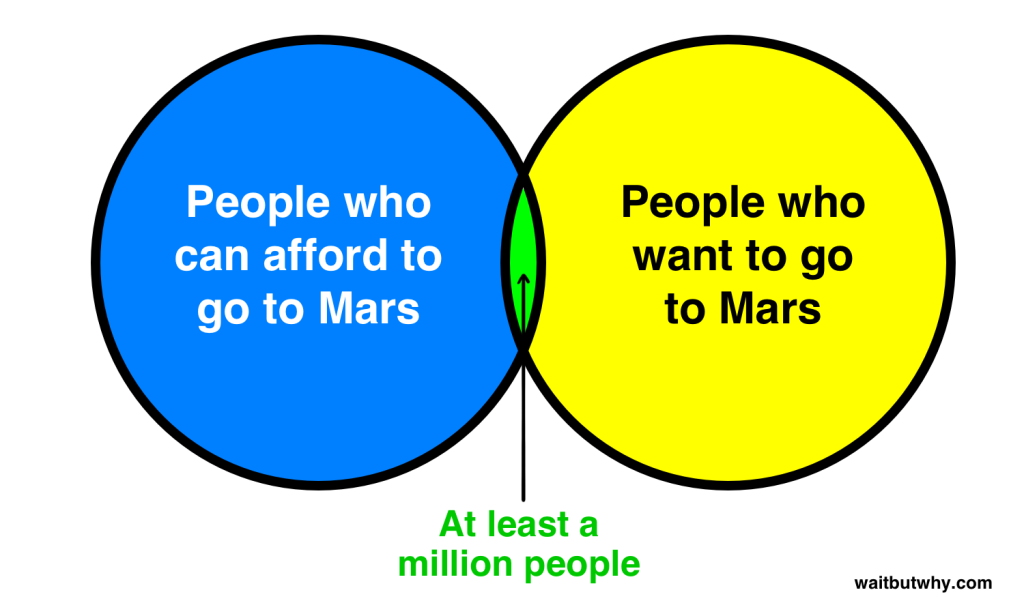
\includegraphics[width=65mm]{images/venn_mars_price}}
        \end{column}
    \end{columns}

\end{frame}
